\section{The Path To Victory 2.0}

A Hamiltonian Path is a path in a graph that visits each vertex exactly once. In this question, we consider the variant of the Hamiltonian Path problem with the start and end node specified: that is, given a graph $G=(V,E)$ and two nodes $s$ and $t$, does there exist a path from $s$ to $t$ that visits every node in $G$ exactly once? You can may assume that $G$ contains at least three vertices.

The Hamiltonian Path problem can be applied to graphs that are either undirected or directed. For example, the undirected graph below has a Hamiltonian Path from A to D given by (A, B, C, D), shown in blue:

\begin{center}
	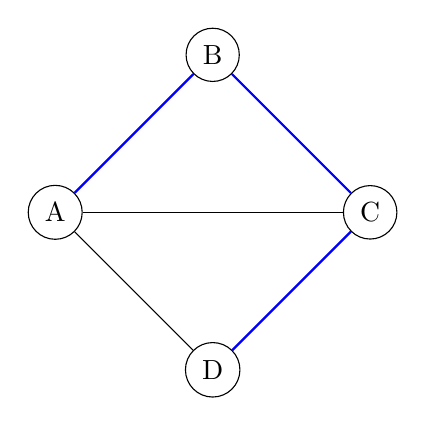
\begin{tikzpicture}
		% Define the vertices
		\node[draw, circle] (A) at (0, 0) {A};
		\node[draw, circle] (B) at (2, 2) {B};
		\node[draw, circle] (C) at (4, 0) {C};
		\node[draw, circle] (D) at (2, -2) {D};

		% Define the edges
		\draw (A) -- (B);
		\draw (B) -- (C);
		\draw (C) -- (D);
		\draw (A) -- (C);
		\draw (A) -- (D);

		% Highlight the Hamiltonian Path A-B-C-D
		\draw[blue, thick] (A) -- (B);
		\draw[blue, thick] (B) -- (C);
		\draw[blue, thick] (C) -- (D);
	\end{tikzpicture}
\end{center}

For the directed graphs below, the graph on the left has a Hamiltonian Path from A to D, while the graph on the right does not have a Hamiltonian Path from A to D.

\begin{center}
	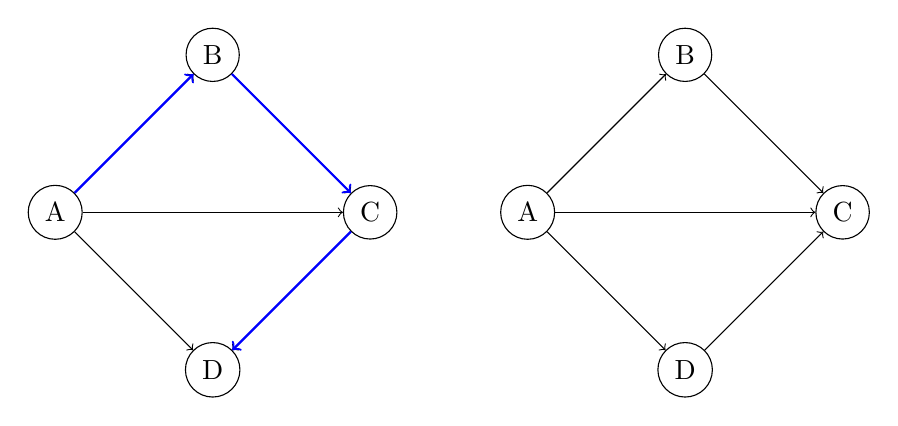
\begin{tikzpicture}
		% First graph with Hamiltonian Path
		\node[draw, circle] (A1) at (0, 0) {A};
		\node[draw, circle] (B1) at (2, 2) {B};
		\node[draw, circle] (C1) at (4, 0) {C};
		\node[draw, circle] (D1) at (2, -2) {D};

		\draw[->] (A1) -- (B1);
		\draw[->] (B1) -- (C1);
		\draw[->] (C1) -- (D1);
		\draw[->] (A1) -- (C1);
		\draw[->] (A1) -- (D1);

		\draw[blue, thick, ->] (A1) -- (B1);
		\draw[blue, thick, ->] (B1) -- (C1);
		\draw[blue, thick, ->] (C1) -- (D1);

		% Second graph without Hamiltonian Path
		\node[draw, circle] (A2) at (6, 0) {A};
		\node[draw, circle] (B2) at (8, 2) {B};
		\node[draw, circle] (C2) at (10, 0) {C};
		\node[draw, circle] (D2) at (8, -2) {D};

		\draw[->] (A2) -- (B2);
		\draw[->] (B2) -- (C2);
		\draw[->] (D2) -- (C2);
		\draw[->] (A2) -- (C2);
		\draw[->] (A2) -- (D2);

	\end{tikzpicture}
\end{center}

We refer to the undirected version of this problem as \textbf{UHP} and the directed version as \textbf{DHP}.

\begin{questions}

	\question[3] Give a reduction from UHP to DHP.

	\ifsolutions\begin{soln}
	Claim: that
\end{soln}
\fi

	\begin{soln}

		Let \(G = (V, E)\) be an undirected graph. We construcut a graph \(G' = (V, E')\) by the following.

		For each \(\{u, v\} \in E\) add \((u, v), (v, u)\) to \(E'\).

		Then for \(s, t \in V\) we ask DHP if there exists a Hamiltonian path from \(s\) to \(t\) in \(G'\).

	\end{soln}


	\question[4] Prove the correctness of your reduction from UHP to DHP. That is, prove that the answer to your reduced DHP instance is YES if and only if the answer to UHP is YES.

	\ifsolutions\begin{soln}
	Let \(P = (v_1, v_2, \dots, v_n)\) be a permutation on \(V\).

	We will assume that we have an adjency matrix to represent the edges in the graph \(M\).

	\begin{algorithmic}[1]
		\Procedure {Valid-Ranking}{P, M}
		\For{each $i = 1, 2, \dots, n - 1$}
		\State store the sum from $j = i$ to $j = n$ of $M(j)$ as $d_i$
		\For{each $j = i + 1, \dots, n - 1$}
		\State store the sum from $k = j$ to $k = n$ of $M(k)$ as $d_k$
		\If{$d_i < d_k$}
		\State end the procedure, report it is not valid
		\EndIf
		\EndFor
		\EndFor
		\State report the permutation as valid
		\EndProcedure
	\end{algorithmic}
	This algorithm is \(O(n^3)\), where \(n = |P|\). In the worse case, we have a valid permutation, and the algorithm does work as follows.

	We have to iterate through the permutation list \(n - 1\) times. Access to the elements will be \(O(1)\) as we assume we are given an array.

	Then for each iteration, we are iterating through the entire adjency matrix, except each iteration we are considering one less node.

	Access to the adjency matrix is \(O(1)\) thus the iteration of the adjency matrix is \(O(i^2)\).

	Then, for each \(i\), the work we are doing is \(i^2\). Thus, summing \(i = 1, 2, \dots, n - 1\) gives us \(O(n^3)\).


\end{soln}
\fi
	\begin{soln}

		We'll say that \(V = \{s, v_1, v_2, \dots, v_{n-2}, t\}\). And we ask for Hamiltonian path from \(s\) to \(t\).

		\((\implies)\): Suppose that the answer to the reduced DHP instance is YES.

		Then there is a Hamiltonian path from \(s-t\) in \(G' = (V, E')\).

		Then there is a simple path on \(V\), \((s, v_1, v_2, \dots, v_{n-2}, t)\) so that \((s, v_1) \in E', (v_{n-2}, t) \in E'\) and \((v_{i},v_{i+1}) \in E'\) for \(i = 1, 2, \dots n - 3\).

		By construction, we have that \(\{s, v_1\}, \{v_{n-2}, t\} \in E\) and \(\{v_i, v_{i+1}\} \in E\) for \(i = 1, 2, \dots, n - 3\).

		By definition, \((s, v_1, v_2, \dots, v_{n- 2}, t)\) is also a simple path in \(G = (V, E)\).

		But this contains all nodes in \(V\), thus it is a Hamiltonian path.

		\((\impliedby)\): Suppose that the answer to UHP is YES for the graph \(G = (V, E)\).

		This means that there is a Hamiltonian path, \((s, v_1, v_2, \dots, v_{n-2}, t)\) so that \(\{s, v_1\}, \{v_{n-2}, t\} \in E\) and \(\{v_i, v_{i+1}\} \in E\) for \(i = 1, 2, \dots, n - 3\).

		We aim to show there exists a Hamiltonian path in the reduction instance.

		For \(G' = (V, E')\), \((s, v_1) \in E', (v_{n-2}, t) \in E'\) and \((v_{i},v_{i+1}) \in E'\) for each \(i = 1, 2, \dots n - 3\) by assumption.

		Then the same path, \((s, v_1, v_2, \dots, v_{n-2}, t)\) is by definition Hamiltonian, since each node in \(V\) appears in it exactly once and the associated directed edges exist.

		This completes the proof.
	\end{soln}

	\question[7] Give a reduction from DHP to UHP. You \textbf{do not} need to prove the correctness of this reduction, but you should clearly explain the key components of your reduction and why they are there.

	\ifsolutions\begin{soln}
	Suppose we are given a tournament graph \(T = (V, E)\) with a vertex ordering \(v_1, v_2, \dots, v_n\) such that for all \(i < j\), the directed edge \((v_i, v_j)\) is in \(E\). That is, every vertex points to all vertices that come after it in the order.

	\textbf{Claim 1:} \(T\) is a tournament.

	For every distinct pair \(v_i, v_j\), either \(i < j\) or \(j < i\), so exactly one of \((v_i, v_j)\) or \((v_j, v_i)\) exists in \(E\), but not both. This satisfies the definition of a tournament: for every pair of distinct vertices, there is exactly one directed edge between them.

	\textbf{Claim 2:} The ordering \(v_1, v_2, \dots, v_n\) is a valid ranking.

	Let \(d_i\) be the out-degree of \(v_i\) in the subtournament induced by \(\{v_i, v_{i+1}, \dots, v_n\}\). Since \(v_i\) points to all vertices that follow it, it has out-degree \(d_i = n - i\). For \(i < j\), \(d_i = n - i > n - j = d_j\), so each player has strictly higher out-degree than those who come after them. Thus, the ordering satisfies the requirement of a valid ranking.

	\textbf{Claim 3:} The valid ranking is unique.

	Suppose for contradiction there is another valid ranking \(P' = v_{\pi(1)}, v_{\pi(2)}, \dots, v_{\pi(n)}\) with \(\pi\) a permutation of \(\{1, \dots, n\}\), and \(P' \ne P\). Then there exist indices \(i < j\) such that \(\pi(i) > \pi(j)\); that is, \(v_{\pi(i)}\) appears before \(v_{\pi(j)}\) in \(P'\), but comes later in the original ordering.

	But then in the subtournament starting at \(v_{\pi(i)}\), the vertex \(v_{\pi(i)}\) must have lower out-degree than \(v_{\pi(j)}\), contradicting the assumption that \(P'\) is a valid ranking. So the valid ranking must be unique.

	Suppose we have a tournament graph \(T = (V, E)\) such that there is an ordering, \(v_1, v_2, \dots, v_n\) so that there is an edge \((v_i, v_j)\) iff \(i < j\).

	This would create one valid ranking, and this ordering is exactly that ranking.

	Before we prove that statement, we will show it is a tournament in the first place, and that is is valid ranking.

	First, we require that every player has played someone else and only once or in other words, either \((v_i, v_j) \in E\) or \((v_j, v_i) \in E\) but not both.

	Let \(v_i, v_j \in V\) such that \(i \neq j\). Then either \(i < j\) or \(j < i\). Then we can only have one of the edge pairs in \(E\) by assumption.

	Next, we require that \(v_i\) has maximum out-degree in its subtournaments.

	Observe that for any \(v_i\) in a subtournament it's out degree is \(d_i = n - i + 1\), independent of the sub tournament.

	Then for any \(i < j\), we see that \(n - j + 1 < n - i + 1\), but this precisely means that \(d_j < d_i\), thus it is valid ranking.

	Proof: For contradiction, suppose that there were two valid rankings.

	Then it must be some permutation on \(P:= v_1, v_2, \dots, v_n\).

	Then there exists some \(i < j\) in \(P\) such that \(j < i\) in \(P'\). But this means that \(d_j < d_i\) in the subtournament for \(j\) in \(P'\).

	This contradicts that \(P'\) was a valid ranking.
\end{soln}
\fi

	\begin{soln}
		Let \(G = (V, E)\) be a directed graph. With \(V = \{s, v_1, v_2, \dots v_{n-2}, t\}\).

		Let \(V_o, V_i\) be vertex sets such that \(|V| = |V_o| = |V_i|\).

		Let \(f_o : V \to V_o\) and \(f_i : V \to V_i\) be bijective functions.

		Here, we make two copies of the vertex set and will encode the directed edge using copies of the nodes.

		We then construct a new edge set \(E'\) based on the original directed edge set \(E\).

		Then for each edge \((v, u) \in E\) we add \(\{f_o(v), f_i(u)\}\) to \(E'\). We also add for each \(v \in V, \{f_o(v), f_i(v)\}\) to \(E'\).

		Then our new graph is \(G' = (V_o \cup V_i, E')\).

		In other words, \(V_o\) corresponds to the original vertices acting as outgoing nodes, and \(V_i\) corresponds to the original vertices acting as incoming nodes.

		As an illustration,

		\begin{center}
			Original Directed Graph
		\end{center}

		\begin{tikzpicture}[->, >=Stealth, node distance=2.5cm, thick]

			\node[circle, draw] (s) {s};
			\node[circle, draw, right of=s] (v) {v};
			\node[circle, draw, right of=v] (t) {t};
			\node[circle, draw, right of=t] (u) {u};

			\draw (s) -- (v);
			\draw (v) -- (t);
			\draw (s) .. controls +(up:1cm) and +(up:1cm) .. (t);
			\draw (v) .. controls +(down:1cm) and +(down:1cm) .. (u);
			\draw (u) -- (t);

		\end{tikzpicture}

		\vspace{1cm}

		\begin{center}
			Reduced Undirected Graph using \(V_o\) and \(V_i\)
		\end{center}

		\begin{tikzpicture}[thick, node distance=2.5cm]

			% Outgoing nodes
			\node[circle, draw] (so) at (0,0) {$s_o$};
			\node[circle, draw] (vo) at (2.5,0) {$v_o$};
			\node[circle, draw] (to) at (5,0) {$t_o$};
			\node[circle, draw] (uo) at (7.5,0) {$u_o$};

			% Incoming nodes
			\node[circle, draw, below=of so] (si) {$s_i$};
			\node[circle, draw, below=of vo] (vi) {$v_i$};
			\node[circle, draw, below=of to] (ti) {$t_i$};
			\node[circle, draw, below=of uo] (ui) {$u_i$};

			% Undirected edges based on directed ones
			\draw (so) -- (ti);
			\draw (so) -- (vi);
			\draw (vo) -- (ti);
			\draw (uo) -- (ti);
			\draw (vo) -- (ui);
			\draw (vo) -- (vi);
			\draw (uo) -- (ui);
			\draw (to) -- (ti);
			\draw (so) -- (si);

		\end{tikzpicture}

		We then ask UHP does there exists a hamiltonian path from \(f_i(s)\) to \(f_o(t)\) in \(G'\)?

		If yes, our original graph has a hamiltonian path, if not, then it does not.

		Proof of Correctness: Say that \(|V| = n\), where \(n \geq 3\).

		Assume DHP returns yes when asked if \(G = (V, E)\) if it contains hamiltonian path from \(s\) to \(t\) in \(V\).

		We show there exists a hamiltonian path in \(G' = (V_i \cup V_o, E')\) so that UHP returns yes on \(f_i(s), f_o(t)\).

		By construction, each of \(\{f_i(v), f_o(v)\} \in E'\). Let \(P = (s, v_1, v_2, \dots, v_{n-2}, t)\) be the hamiltonian path.

		By definition, \((s, v_1), (v_{n-2}, t) \in E\) and \((v_i, v_{i+1}) \in E\) for \(i = 1, 2, \dots, n - 3\).

		Then consider the permutation of nodes on \(V_o \cup V_i\), by the following:

		\(P' = (f_i(s), f_o(s), f_i(v_1), f_o(v_1), f_i(v_2), f_o(v_2), \dots f_i(v_{n-2}), f_o(v_{n-2}), f_i(t), f_o(t))\).

		By construction, \(\{f_o(s), f_i(v_1)\}, \{f_o(v_{n-2}), f_i(t))\} \in E'\). As those directed edges exist in that order.

		Similarly, \(\{f_o{v_i}, f_i(v_{i+2})\} \in E'\) for \(i = 1, 2, \dots, n - 3\). But by definition, \(P'\) is a hamiltonian path in \(G'\).

		Thus, UHP will return yes when asked if \(G'\) contains a hamiltonian path from \(f_i(s)\) to \(f_o(t)\).

		This proves one direction, now assume that UHP returns yes upon begin given \(G' = (V_i \cup V_o, E')\).

		We will show that this means there is a hamiltonian path in \(G\) from \(s\) to \(t\).

		Observe that for any \((u, v) \in E\) that \(\{f_o(u),f_o(v)\}, \{f_i(u), f_i(v)\} \notin E'\) by construction.

		In other words, the outcoming nodes do not connect to each other and the the incoming nodes do not connect to each other in \(G'\).

		Thus, for any path in \(G'\) of the form, \(\rho = (v_1,v_2, \dots, v_k)\) if \(v_j \in V_o\) then \(v_{j+1} \in V_i\) for \(j = 1, 2, \dots, k - 1\).

		Let \(P = (f_i(s), o_1, i_1, o_2, i_2, \dots, o_{n-1}, i_{n-1}, f_o(t))\) be the hamiltonian path from \(f_o(s)\) to \(f_i(t)\) in \(G'\) such that \(i_j \in V_i, o_j \in V_j\).

		Now construct, \(P' = \)





	\end{soln}


\end{questions}
